\documentclass{beamer}
\usepackage{minted}
\usepackage{epigraph}
\usepackage{subfig}
\usepackage{pgfplots}
\usepackage{tikz}
\usepackage{color, colortbl}

\usetheme{focus}

\definecolor{orangered}{rgb}{1,0.45, 0}

\title{Shell Linux \& BASH scripting}
\subtitle{Tutorato Sistemi Operativi}
\author{Davide Carnemolla}
\titlegraphic{
\includegraphics[scale=0.13]{images/penguin2.pdf}}
\institute{Dipartimento di Matematica e Informatica \\ Università di Catania}
\date{2022/2023}

\begin{document}
    \begin{frame}
        \maketitle
    \end{frame}

    \begin{frame}{\$ whoami}
        \centering
        \begin{tikzpicture} 
            \begin{scope}
                \clip [rounded corners=1.25cm] (0,0) rectangle coordinate (centerpoint) (2.5,2.5cm); 
                \node [inner sep=0pt] at (centerpoint) {
\includegraphics[width=2.5cm, keepaspectratio]{images/dc.jpg}}; 
            \end{scope}
        \end{tikzpicture}

        \textbf{Davide Carnemolla} \\ @Herbrant

        \vspace{1cm}

        \begin{columns}[t, onlytextwidth]
            \column{0.33\textwidth}
                \centering
                
\includegraphics[height=1.5cm, keepaspectratio]{images/open-source.pdf}

                \small Open Source Enthusiast
               

            \column{0.33\textwidth}
                \centering
                
\includegraphics[height=1.5cm, keepaspectratio]{images/exambox.pdf}

                \small ExamBox's father
            
            \column{0.33\textwidth}
                \centering
                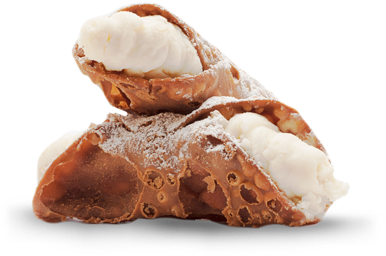
\includegraphics[height=1.5cm, keepaspectratio]{images/cannoli.png}

                \small Ricotta lover
    
        \end{columns}        
    \end{frame}
    
    \section{Shell Linux}

    \begin{frame}{La Shell}
        \begin{columns}[t, onlytextwidth]
            \column{0.2\textwidth}
                \centering
                
\includegraphics[height=2.5cm, keepaspectratio]{images/user.pdf}

            \column{0.2\textwidth}
                \centering
                
\includegraphics[height=2cm, keepaspectratio]{images/rightarrow.pdf}
            
            \column{0.2\textwidth}
                \centering
                
\includegraphics[height=2.5cm,keepaspectratio]{images/terminal.pdf}

            \column{0.2\textwidth}
                \centering
                
\includegraphics[height=2cm, keepaspectratio]{images/rightarrow.pdf}

            \column{0.2\textwidth}
                \centering
                
\includegraphics[height=2.5cm, keepaspectratio]{images/linux.pdf}
        \end{columns}
    \end{frame}

    \begin{frame}{Il filesystem}
        \centering
        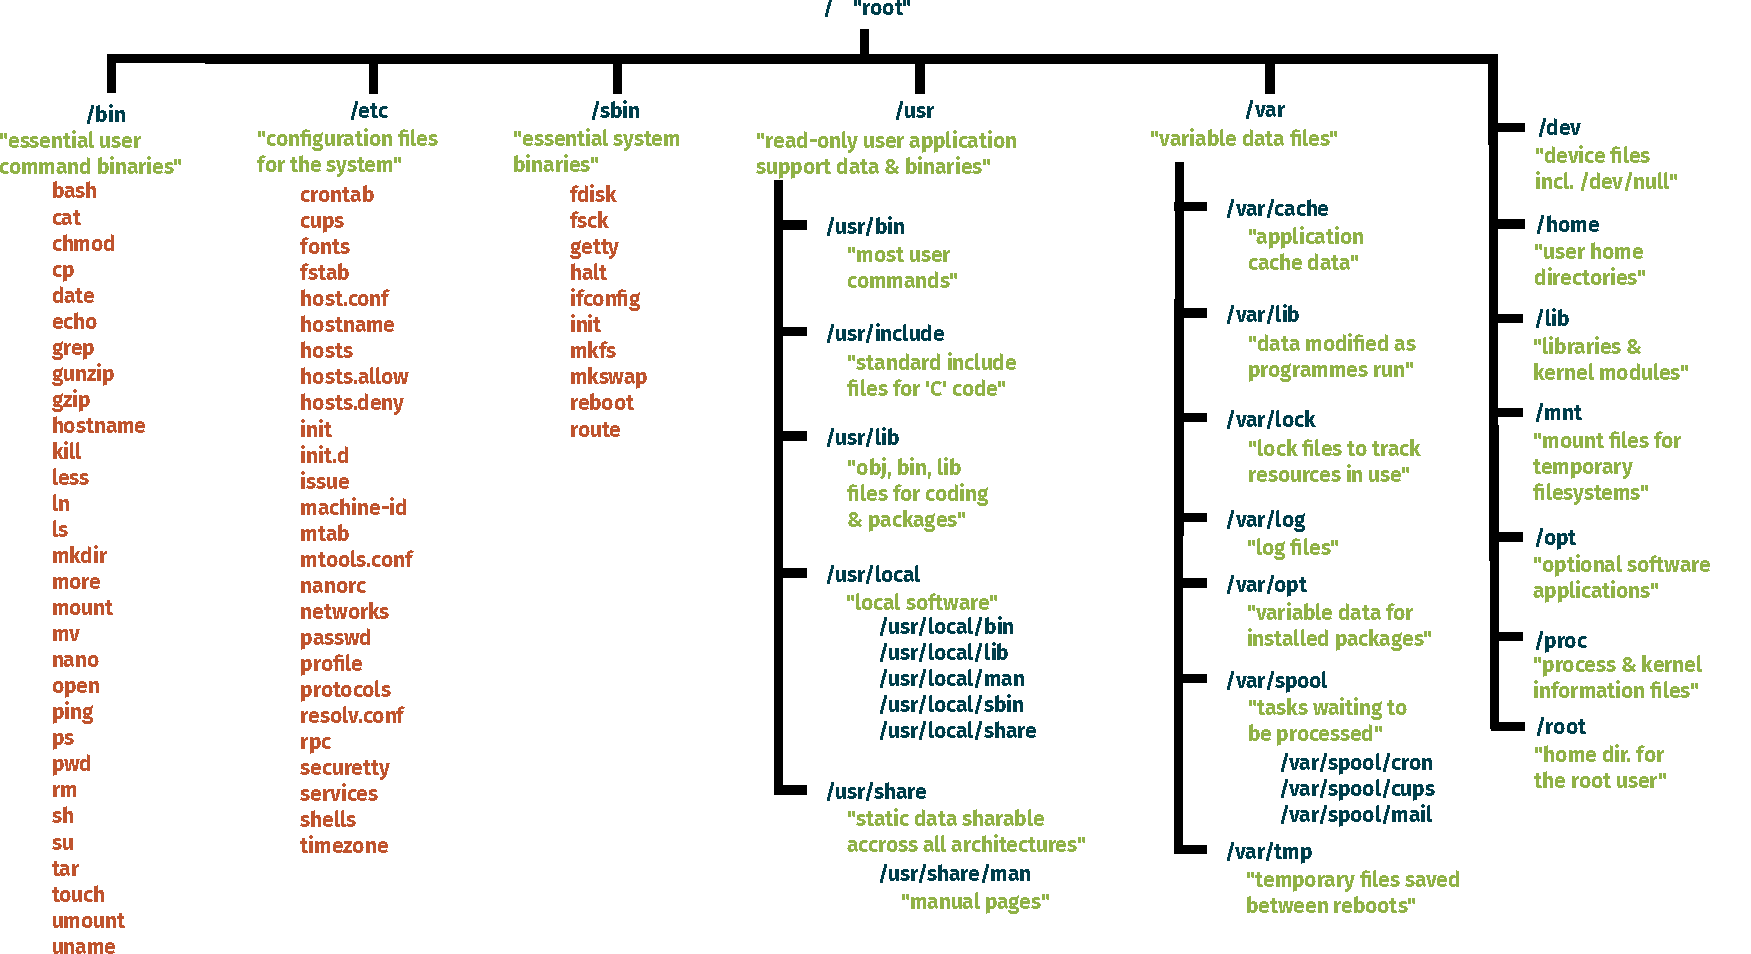
\includegraphics[height=6cm, keepaspectratio]{images/unix-fs.pdf}
    \end{frame}

    \begin{frame}{I Path}
        \centering
        
\includegraphics[height=2cm, keepaspectratio]{images/path.pdf}
        \vspace{0.5cm}
        \begin{block}{Path assoluto}
            Il \textbf{percorso assoluto} di un file è il percorso
            che va dalla radice del filesystem allo stesso.
        \end{block}

        \begin{block}{Path relativo}
            Fissando logicamente una particolare directory (in genere quella corrente) è possibile identificare un file attraverso il
            \textbf{percorso relativo} che va da tale directory ad esso.
        \end{block}
    \end{frame}

    \begin{frame}{I Path}
        \begin{alertblock}{Nota}
            Il percorso assoluto di un file è il suo percorso relativo rispetto
            alla root.
        \end{alertblock}

        \begin{exampleblock}{Esempio}
            \textbf{Directory corrente}: \texttt{/home/}

            \textbf{Path assoluto}: \texttt{/home/davide/file.txt}

            \textbf{Path relativo}: \texttt{davide/file.txt}
        \end{exampleblock}

        \begin{block}{Cartelle virtuali}
            \begin{itemize}
                \item la cartella \texttt{.} indica la cartella stessa
                \item la cartella \texttt{..} indica la cartella genitore (utile per navigare il filesystem)
            \end{itemize}
        \end{block}
    \end{frame}

    \begin{frame}{Path: file di dispositivo}
        In ambiente UNIX esistono dei file speciali chiamati file di dispositivo:
        identificano una particolare periferica del sistema ed attraverso questo è possibile interagire con tale periferica. \\
        \vspace{0.25cm}
        \begin{columns}[t, onlytextwidth]
            \column{0.5\textwidth}
                \centering
                
\includegraphics[height=1.5cm, keepaspectratio]{images/char.pdf}
                
                \textbf{A caratteri}

            \column{0.5\textwidth}
                \centering
                
\includegraphics[height=1.5cm, keepaspectratio]{images/block.pdf}
                
                \textbf{A blocchi}
        \end{columns}

        \vspace{0.25cm}

        \begin{exampleblock}{Esempi}
            \begin{itemize}
                \item \texttt{/dev/sda,/dev/sdb}\dots
                \item \texttt{/dev/sda1,/dev/sda2}\dots
                \item \texttt{/dev/tty1,/dev/tty2}\dots
            \end{itemize}
        \end{exampleblock}
    \end{frame}

    \begin{frame}{Path: pseudo-devices}
        \begin{columns}[t, onlytextwidth]
            \column{0.33\textwidth}
                \centering
                
\includegraphics[height=2cm, keepaspectratio]{images/dice.pdf}
                
                \texttt{\textbf{/dev/random}}
            \column{0.33\textwidth}
                \centering
                
\includegraphics[height=2cm, keepaspectratio]{images/ram.pdf}
                
                \texttt{\textbf{/dev/shm}}
            \column{0.33\textwidth}
                \centering
                
\includegraphics[height=2cm, keepaspectratio]{images/hole.pdf}
                \texttt{\textbf{/dev/null}}
        \end{columns}

        \vspace{2cm}

        \begin{columns}[t, onlytextwidth]
            \column{0.5\textwidth}
                \centering
                
\includegraphics[height=2cm, keepaspectratio]{images/alert-file.pdf}

                \texttt{\textbf{/dev/full}}
            \column{0.5\textwidth}
                \centering
                
\includegraphics[height=2cm, keepaspectratio]{images/terminal.pdf}

                \texttt{\textbf{/dev/ttyX}}
        \end{columns}
        
    \end{frame}

    \begin{frame}{Mount: quando voglio più spazio}
        \centering
        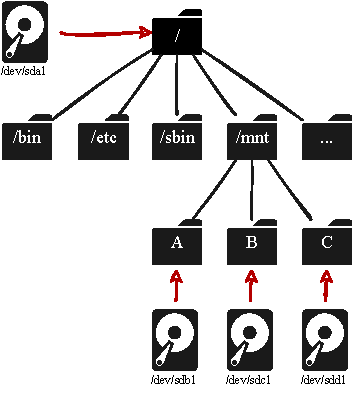
\includegraphics[height=7.5cm, keepaspectratio]{images/mountpoint.pdf}
    \end{frame}

    \begin{frame}{Hello Shell}
        \begin{exampleblock}{}
            \texttt{\$ echo "Hello shell"}
        \end{exampleblock}

        \begin{itemize}
            \item \textbf{echo} rappresenta il comando
            \item \textbf{"Hello world"} rappresenta un parametro per il comando
        \end{itemize}

        \begin{block}{Parametri}
            Tipicamente un comando richiede dei parametri
            
            \vspace{0.5cm}

            \begin{columns}[t, onlytextwidth]
                \column{0.33\textwidth}
                    \centering
                    
\includegraphics[height=1cm, keepaspectratio]{images/file.pdf}
                    
                    \textbf{File}
    
                \column{0.33\textwidth}
                    \centering
                    
\includegraphics[height=1cm, keepaspectratio]{images/input-data.pdf}
                    
                    \textbf{Dati}
                \column{0.33\textwidth}
                    \centering
                    
\includegraphics[height=1cm, keepaspectratio]{images/options.pdf}
                    
                    \textbf{Opzioni}
            \end{columns}

            \vspace{0.5cm}
        \end{block}
    \end{frame}

    \begin{frame}{Comandi utili}
        \begin{columns}[t, onlytextwidth]
            \column{0.33\textwidth}
                \centering
                \Huge \textbf{CTRL + C}
                
                \vspace{0.2cm}
                
                \normalsize \textit{``No maria, io esco''}
            \column{0.33\textwidth}
                \centering
                \Huge \textbf{CTRL + S}

                \vspace{0.2cm}

                \normalsize \textit{``Finisco di mangiare la peperonata e scendo! ''}
            \column{0.33\textwidth}
                \centering
                \Huge \textbf{CTRL + Q}

                \vspace{0.2cm}

                \normalsize \textit{``Ok ho digerito: possiamo riprendere.''}
        \end{columns}
    \end{frame}

    \begin{frame}{Comandi utili}
        \centering
        
\includegraphics[height=4cm,keepaspectratio]{images/spongebob-crying.png}

        \Large \textit{``Non riesco a fare copia e incolla''}
        
        \vspace{1cm}

        \begin{columns}[t, onlytextwidth]
            \column{0.5\textwidth}
                \centering
                \huge \textbf{CTRL+SHIFT+C}
            \column{0.5\textwidth}
                \centering
                \huge \textbf{CTRL+SHIFT+V}
        \end{columns}
    \end{frame}

    \begin{frame}{Hello man}
        \begin{columns}[t, onlytextwidth]
            \column{0.33\textwidth}
                \centering
                
\includegraphics[height=2cm]{images/search.pdf}

                \vspace{0.2cm}

                \textit{apropos stringa}
            \column{0.33\textwidth}
                \centering
                
\includegraphics[height=2cm]{images/whatis.pdf}

                \vspace{0.2cm}

                \textit{whatis stringa}
            \column{0.33\textwidth}
                \centering
                
\includegraphics[height=2cm]{images/man.pdf}

                \vspace{0.2cm}

                \textit{man stringa}
        \end{columns}
    \end{frame}

    \begin{frame}{Warning}
        \centering
        
\includegraphics[height=3cm, keepaspectratio]{images/warning.pdf}

        \vspace{0.5cm}

        \Large La sintassi dei comandi presentati è stata semplificata per facilitare la presentazione

        \vspace{0.5cm}

        \small Per maggiori informazioni consultare sempre il manuale (\texttt{\textbf{man}})
    \end{frame}

    \begin{frame}{Filesystem: ls}
        \begin{block}{ls}
            Sintassi: \texttt{\textbf{ls [-l] [-a] [-R] [pathname\dots]}}

            \begin{itemize}
                \item \texttt{\textbf{-l}}: visualizza informazioni dettagliate
                \item \texttt{\textbf{-a}}: visualizza anche i file nascosti
                \item \texttt{\textbf{-R}}: visualizza il contenuto delle cartelle ricorsivamente
                \item \texttt{\textbf{pathname}}: oggetto del filesystem sul quale visualizzare le informazioni
            \end{itemize}
        \end{block}

        \begin{exampleblock}{Esempio}
            \$ ls /home/davide/script.sh
            
            -rwxr-{}-r-{}- 1 davide davide 967 31 mag 23.05 script.sh
        \end{exampleblock}
    \end{frame}

    \begin{frame}{Permessi di accesso}
        Nei sistemi Unix ogni file possiede dei permessi di accesso.

        In principali sono:
        \begin{itemize}
            \item \textbf{r}: lettura
            \item \textbf{w}: scrittura
            \item \textbf{x}: esecuzione/attraversamento (directory)
        \end{itemize}

        \vspace{0.5cm}

        Inoltre, il primo carattere è destinato a dei flag speciali:
        \begin{itemize}
            \item \textbf{d}: si tratta di una directory
            \item \textbf{l}: si tratta di un soft link
            \item \textbf{s}: attribuisce al file in esecuzione i privilegi dell'utente cui appartiene (SUID)
        \end{itemize}

        \begin{exampleblock}{Esempio}
            -rwxr-{}-r-{}- 1 davide davide 967 31 mag 23.05 script.sh
        \end{exampleblock}
    \end{frame}

    \begin{frame}{I metacaratteri}
        Per abbreviare il nome di un file da specificare o per specificarne più di uno
        si possono utilizzare i metacaratteri:
        \begin{itemize}
            \item \textbf{*}: rappresenta una qualunque stringa di 0 o più caratteri
            \item \textbf{?}: rappresenta un qualsiasi carattere
            \item \textbf{[]}: singolo carattere tra quelli elencati
            \item \textbf{\{\}}: singola stringa tra quelle elencate
        \end{itemize}
        \begin{exampleblock}{Esempio}
            \footnotesize

            \$ ls

            esempio2.txt esempio3.txt esempio.txt script.sh scheda.pdf

            \vspace{0.25cm}

            \$ ls esempio*.txt

            esempio2.txt esempio3.txt esempio.txt

            \vspace{0.25cm}

            \$ ls esempio?.txt

            esempio2.txt esempio3.txt esempio.txt

            \vspace{0.25cm}

            \$ ls *.\{txt,pdf\}

            esempio2.txt esempio3.txt esempio.txt scheda.pdf
        \end{exampleblock}
    \end{frame}

    \begin{frame}{Filesystem: cd/pwd}
        \begin{block}{cd}
            \small
            Sintassi: \texttt{\textbf{cd [pathname]}}
            
            \begin{itemize}
                \item \textbf{pathname}: nuova directory corrente (assoluto o relativo)
            \end{itemize}

            Il comando ci permette di navigare all'interno del
            filesystem cambiando di volta in volta la directory corrente.
        \end{block}

        \begin{block}{pwd}
            \small
            Sintassi: \texttt{\textbf{pwd}}

            Il comando ci permette di ottenere la \textit{present working directory}, ovvero il path assoluto
            della directory in cui ci troviamo.
        \end{block}
    \end{frame}

    \begin{frame}{Filesystem: mkdir/rmdir}
        \begin{block}{mkdir}
            \small
            Sintassi: \texttt{\textbf{mkdir [-p] pathname\dots}}

            \begin{itemize}
                \item \texttt{\textbf{-p}}: non restituisce errori se la directory esiste già e crea tutte le directory necessarie per ottenere il path completo
                \item \texttt{\textbf{pathname}}: pathname da creare
            \end{itemize}

            Il comando \textbf{mkdir} crea le directory specificate mediante i parametri.
        \end{block}

        \begin{block}{rmdir}
            \small
            Sintassi: \texttt{\textbf{rmdir [-p] pathname\dots}}

            \begin{itemize}
                \item \textbf{-p}: rimuove tutte le directory presenti nel pathname
                \item \textbf{pathname}: directory da eliminare
            \end{itemize}

            Il comando \textbf{rmdir} rimuove una directory vuota dal filesystem.
        \end{block}
    \end{frame}

    \begin{frame}{Filesystem: cp}
        \centering
        
\includegraphics[height=2.5cm, keepaspectratio]{images/spider-man-meme.jpg}

        \begin{block}{cp}
            \small
            Sintassi: \texttt{\textbf{cp [-R] [-i] source... dest}}

            \begin{itemize}
                \item \textbf{-R}: copia ricorsivamente il contenuto di una directory
                \item \textbf{-i}: chiede conferma prima di sovrascrivere i file
                \item \textbf{source}: oggetti da copiare
                \item \textbf{dest}: destinazione in cui copiare gli oggetti
            \end{itemize}

            Il comando \textbf{cp} copia i file specificati con \textbf{source} in \textbf{dest}.
        \end{block}
    \end{frame}

    \begin{frame}{Filesystem: rm}
        \centering
        
\includegraphics[height=3cm, keepaspectratio]{images/willy.jpg}

        \begin{block}{rm}
            \small
            Sintassi: \texttt{\textbf{rm [-r] [-i] [-f] pathname...}}

            \begin{itemize}
                \item \textbf{-r}: elimina ricorsivamente tutti i file
                \item \textbf{-i}: chiede conferma prima di cancellare ogni file
                \item \textbf{-f}: cancella gli oggetti senza chiedere conferma
                \item \textbf{pathname}: oggetti da eliminare
            \end{itemize}

            Il comando \textbf{rm} elimina tutti i file specificati con i parametri.
        \end{block}
    \end{frame}

    \begin{frame}{}
        \centering
        \Huge \texttt{rm -rf /}
    \end{frame}

    \begin{frame}{Filesystem: mv}
        \centering
        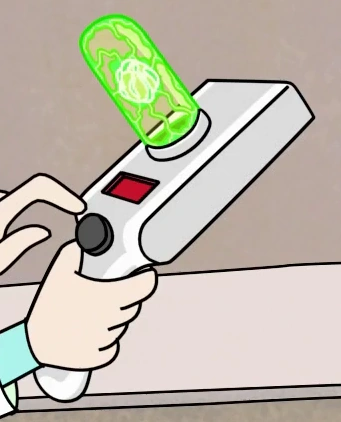
\includegraphics[height=3cm, keepaspectratio]{images/spara-porte.png}

        \begin{block}{mv}
            \small
            Sintassi: \texttt{\textbf{mv source... dest}}

            \begin{itemize}
                \item \textbf{source}: file o directory da spostare
                \item \textbf{dest}: file o directory di destinazione
            \end{itemize}

            Il comando \textbf{mv} sposta il file o directory sorgente nella destinazione specificata.
        \end{block}
    \end{frame}

    \begin{frame}{Filesystem: mount}
        \begin{block}{mount}
            \small
            Sintassi: \texttt{\textbf{mount [-t fstype] [-o options] device mountpoint}}

            \begin{itemize}
                \item \texttt{\textbf{-t fstype}}: permette di specificare il tipo del filesystem da montare (ext2, ext3, ext4, btrfs...)
                \item \texttt{\textbf{-o options}}: permette di specificare ulteriori opzioni per il mount
                \item \texttt{\textbf{device}}: il dispositivo da montare (di solito una partizione del tipo \texttt{/dev/sdaX})
                \item \texttt{\textbf{mountpoint}}: directory in cui montare filesystem
            \end{itemize}

            Il comando \texttt{\textbf{mount}} permette di montare un filesystem all'interno
            dell'albero principale.
        \end{block}
    \end{frame}

    \begin{frame}{Utenti nei sistemi Unix}
        \begin{columns}[t, onlytextwidth]
            \column{0.33\textwidth}
                \centering
                
\includegraphics[height=2.5cm, keepaspectratio]{images/root.pdf}

                \large \textbf{root}
            \column{0.33\textwidth}
                \centering
                \Huge $\longleftarrow$

                \large sudo
            \column{0.33\textwidth}
                \centering
                
\includegraphics[height=2.5cm, keepaspectratio]{images/user2.pdf}

                \large \textbf{standard user}
        \end{columns}
    \end{frame}

    \begin{frame}{}
        \centering
        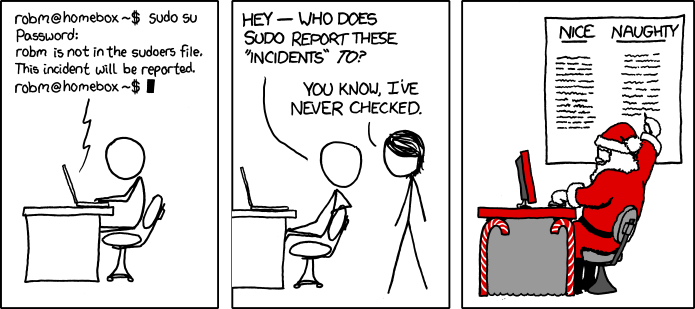
\includegraphics[height=4.5cm, keepaspectratio]{images/sudo-incident.png}
    \end{frame}

    \begin{frame}{Filesystem: chmod}
        \begin{block}{chmod}
            \small
            Sintassi: \texttt{\textbf{chmod [-R] mode [pathname...]}}

            \begin{itemize}
                \item \textbf{-R}: applica i permessi ricorsivamente
                \item \textbf{mode}: nuova maschera dei permessi
                \item \textbf{pathname}: oggetti a cui applicare la nuova maschera
            \end{itemize}

            Il comando \textbf{chmod} permette di cambiare i permessi dei file.
        \end{block}

        \begin{alertblock}{mode: sintassi numerica}
            \small
            \texttt{rw-r-{}-{}-{}-{}- $\rightarrow$ 110 100 000 $\rightarrow$ 640}

            \texttt{rwxr-xr-x $\rightarrow$ 111 101 101 $\rightarrow$ 755}
        \end{alertblock}

        \begin{alertblock}{mode: sintassi simbolica}
            \small
            \texttt{rw-r-{}-{}-{}-{}- $\leftrightarrow$ u=rw,g=r,o-rwx}
        
            \texttt{rw-rw-rw- $+$ u+x,o-rw $\rightarrow$ rwxrw-{}-{}-{}-}
        \end{alertblock}
    \end{frame}

    \begin{frame}{}
        \centering
        
\includegraphics[height=4cm, keepaspectratio]{images/bugs-bunny-communist.png}
        
        \vspace{0.5cm}
        
        \Large \texttt{chmod 777 file.txt}
    \end{frame}

    \begin{frame}{Filesystem: chown}
        \centering
        
\includegraphics[height=3cm, keepaspectratio]{images/bugs-bunny-capitalist.png}
        \begin{block}{chown}
            \small
            Sintassi: \texttt{\textbf{chown [-R] owner[:group] [pathname...]}}

            \begin{itemize}
                \item \texttt{\textbf{-R}}: esegue ricorsivamente le modifiche di proprietà
                \item \texttt{\textbf{owner}}: il nuovo proprietario
                \item \texttt{\textbf{group}}: il nuovo gruppo proprietario
                \item \texttt{\textbf{pathname}}: oggetti a cui vogliamo cambiare la proprietà
            \end{itemize}
        \end{block}
    \end{frame}

    \begin{frame}{}
        \centering
        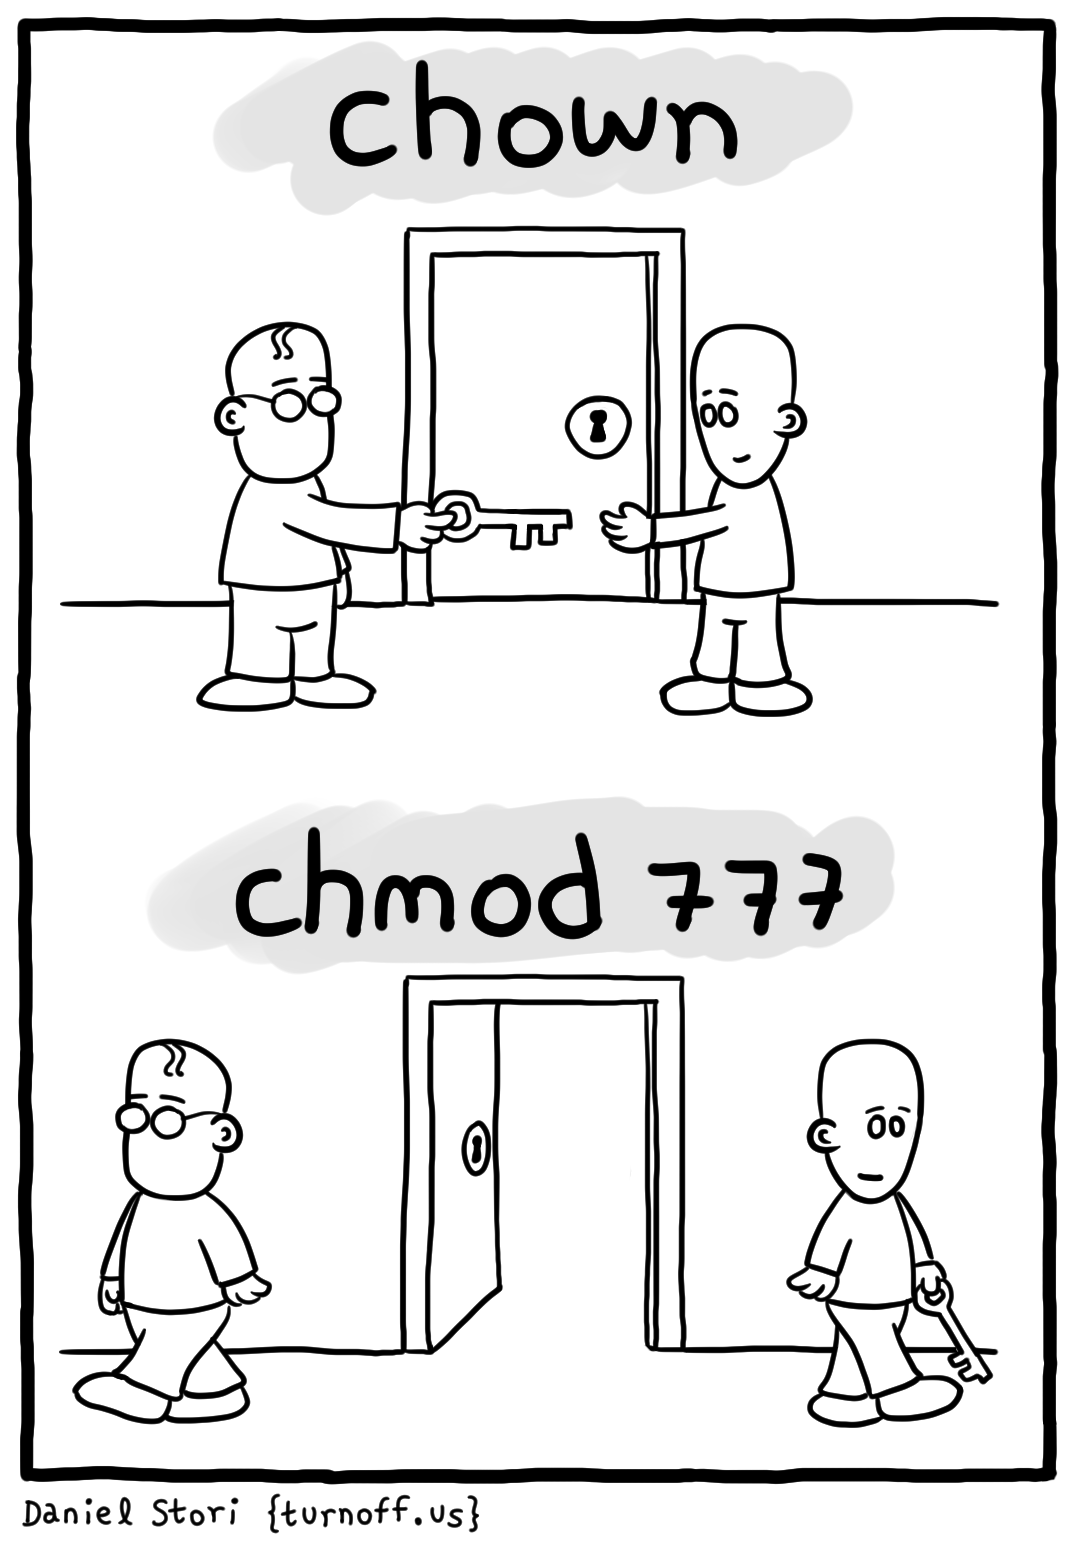
\includegraphics[height=8cm, keepaspectratio]{images/chown-chmod.png}
    \end{frame}

    \begin{frame}{Filesystem: link}
        I filesystem UNIX permettono di creare dei file ``puntatori'' ad oggetto del filesystem, questi sono detti \textbf{link}.
        \begin{alertblock}{Soft link}
            \small
            I \textbf{soft link} (o \textbf{link simbolici}) sono dei file
            speciali che contengono al loro interno il pathname per raggiungere il \textbf{file target}.

            Chiaramente, se viene rimosso il file target, il soft link diventa inconsistente.
        \end{alertblock}

        \begin{alertblock}{Hard link}
            \small

            Gli \textbf{hard link} (o \textbf{link fisici}) agiscono a livello del filesystem. In particolare,
            quando creiamo un hard link creiamo un puntatore all'\textbf{inode} presente nel filesystem.

            Tale operazione è quindi trasparente a livello applicativo.
            
            Non è possibile, per ovvi motivi, creare hard link in filesystem differenti.
        \end{alertblock}
    \end{frame}

    \begin{frame}{Filesystem: ln/readlink}
        \begin{block}{ln}
            \small
            Sintassi: \texttt{\textbf{ln [-s] target... [linkpathname]}}

            \begin{itemize}
                \item \texttt{\textbf{-s}}: crea un link simbolico invece che uno fisico
                \item \texttt{\textbf{target}}: file o directory a cui il link farà riferimento
                \item \texttt{\textbf{linkpathname}}: pathname del link
            \end{itemize}

            Il comando \texttt{\textbf{ln}} consente di creare link tra i file e le directory presenti nel filesystem.
        \end{block}

        \begin{block}{readlink}
            \small
            Sintassi: \texttt{\textbf{readlink pathfile...}}

            \begin{itemize}
                \item \texttt{\textbf{pathfile}}: il path del link simbolico da risolvere
            \end{itemize}

            Il comando \textbf{readlink} restituisce in output la risoluzione del link simbolico.
        \end{block}
    \end{frame}

    \begin{frame}{Filesystem: find}
        \centering
        
\includegraphics[height=3cm, keepaspectratio]{images/scooby.jpg}

        \begin{block}{find}
            \small
            Sintassi: \texttt{\textbf{find [pathname...] [expression]}}

            \begin{itemize}
                \item \texttt{\textbf{pathname}}: percorso in cui cercare ricorsivamente i file
                \item \texttt{\textbf{expression}}: le regole di selezione del file:
                \begin{itemize}
                    \item \texttt{\textbf{optione}}: modifica il comportamento della ricerca
                    \item \texttt{\textbf{condizione}}: condizioni da verificare
                    \item \texttt{\textbf{azione}}: specifica cosa deve fare quando trova il file
                \end{itemize}
            \end{itemize}

            Ricerca nei pathname i file che soddisfano le espressioni date
        \end{block}
    \end{frame}

    \begin{frame}{Filesystem: find}
        \small
        \begin{exampleblock}{Esempio}
            \texttt{\$ find . - name `*.sh' - print \\}
            \texttt{./script.sh \\
            ./prova.sh \\
            ./conta.sh \\
            ./cartella/esercizio/eseguimi.sh}

            \vspace{0.5cm}

            \texttt{\$ find /home/davide -name `*.bak' -exec rm {} \;}
            
            \vspace{0.5cm}

            \texttt{\$ find /etc/ -type d -print}
            \texttt{
                /etc \\
                /etc/pacman.d \\
                /etc/pacman.d/gnupg \\
                /etc/pacman.d/gnupg/private-keys-v1.d \\
                /etc/pacman.d/gnupg/openpgp-revocs.d \\
                ...
            }

        \end{exampleblock}
    \end{frame}

    \begin{frame}{echo}
        \centering
        
\includegraphics[height=3cm, keepaspectratio]{images/george.png}

        \begin{block}{echo}
            \small
            Sintassi \texttt{\textbf{echo [-n] [-e] [stringa...]}}

            \begin{itemize}
                \item \textbf{-n}: non aggiunge l'endline al termine della stringa
                \item \textbf{-e}: permette l'uso di alcuni caratteri speciali
                \item \texttt{\textbf{stringa}}: stringa da visualizzare
            \end{itemize}

            Il comando \texttt{\textbf{echo}} da in output una stringa passata come parametro.
        \end{block}

        
    \end{frame}

    \begin{frame}{cat}
        \centering
        
\includegraphics[height=3cm, keepaspectratio]{images/garfield.jpg}

        \begin{block}{cat}
            \small
            Sintassi: \texttt{\textbf{cat [pathname...]}}

            \begin{itemize}
                \item \texttt{\textbf{pathname}}: file da visualizzare
            \end{itemize}

            Il comando \texttt{\textbf{cat}} permette di mandare allo standard output il contenuto di uno o più file.
        \end{block}
    \end{frame}

    \begin{frame}{more \& less}
        \small
        \begin{block}{more}
            Sintassi: \texttt{\textbf{more [pathname...]}}

            \begin{itemize}
                \item \texttt{\textbf{pathname}}: file da visualizzare
            \end{itemize}

            Il comando \texttt{\textbf{more}} si comporta come \texttt{\textbf{cat}} con
            l'eccezione che se l'output è più lungo di una videata di schermo, ad ogni pagina viene fatta una pausa.
        \end{block}

        \begin{block}{less}
            Sintassi: \texttt{\textbf{less [pathname...]}}

            \begin{itemize}
                \item \texttt{\textbf{pathname}}: file da visualizzare
            \end{itemize}

            Il comando \texttt{\textbf{less}} è una versione più evoluta di \texttt{\textbf{more}}: non solo permette di
            fare pause ad ogni pagina, ma permette anche di andare su e giù
            nell’output. Inoltre è possibile effettuare ricerche interattive
            all’interno del file.
        \end{block}
    \end{frame}

    \begin{frame}{Redirezione dell'I/O}
        Ogni processo ha 3 flussi di dati:

        \begin{itemize}
            \item \textbf{standard input}: da cui prende il suo input; in genere corrisponde alla tastiera
            \item \textbf{standard output}: a cui invia il suo output; in genere corrisponde al terminale video
            \item \textbf{standard error}: a cui invia gli eventuali messaggi d'errore; anche qui si usa in genere il terminale
        \end{itemize}

        Attraverso l'invocazione da riga di comando è possibile
        redirezionare talu flussi su altri file.

        \begin{itemize}
            \item \texttt{\textbf{>}}: redireziona l'output su un file
            \item \texttt{\textbf{<{}<}}: redireziona l'output su un file in modalità \textbf{append}
            \item \texttt{\textbf{<}}: prende l'input da un file
            \item \texttt{\textbf{2>}}: redireziona lo standard error su un file
        \end{itemize}
    \end{frame}

    \begin{frame}{Redirezione dell'I/O: esempi}
        \small

        \begin{exampleblock}{}
            \texttt{\$ ls > output.txt}

            \texttt{\$ cat output.txt}

            \texttt{esempio2.txt esempio3.txt esempio.txt}

            \vspace{0.25cm}

            \texttt{\$ echo Ciao >> output.txt}

            \texttt{\$ cat output.txt}

            \texttt{esempio2.txt esempio3.txt esempio.txt \\ Ciao}

            \vspace{0.25cm}
            
            \texttt{\$ cat < output.txt}

            \texttt{esempio2.txt esempio3.txt esempio.txt \\ Ciao}

            \texttt{\$ man comandochenonesiste}

            \texttt{Non c'è il manuale per comandochenonesiste}

            \vspace{0.25cm}

            \texttt{\$ man comandochenonesiste 2> /dev/null}

            \vspace{0.05cm}
        \end{exampleblock}
    \end{frame}

    \begin{frame}{grep}
        \begin{block}{grep}
            \small
            Sintassi \texttt{\textbf{grep [-i] [-l] [-v] [-w] [pattern] [filename]}}

            \begin{itemize}
                \item \texttt{\textbf{-i}}: ignora le differenze tra maiuscole e minuscole
                \item \texttt{\textbf{-l}}: fornisce la lista dei file che contengono il \texttt{\textbf{pattern}}
                \item \texttt{\textbf{-v}}: stampa le linee che \textbf{non} contengono il \texttt{\textbf{pattern}}
                \item \texttt{\textbf{-w}}: vengono restituite le linee che contengono il \texttt{\textbf{pattern}} come parola completa
                \item \texttt{\textbf{pattern}}: espressione da ricercare
                \item \texttt{\textbf{filename}}: file da analizzare
            \end{itemize}

            Cerca all’interno delle righe dei file specificato le righe che
            contengono (o meno, a secondo delle opzioni) il pattern specificato. Il pattern
            può essere una semplice stringa o una regular expression.
        \end{block}
    \end{frame}

    \begin{frame}{Espressioni regolari}
        Attraverso le \textbf{espressioni regolari} è possibile specificare dei
        \textit{pattern} più complessi della semplice stringa contenuta.

        \begin{center}
            \begin{tabular}{ |c|c| } 
                \hline
                \textbf{metacarattere} & \textbf{significato} \\
                \hline 
                $\hat{}$ & \small inizio della linea \\ 
                \hline
                \$ & \small fine della linea \\
                \hline 
                . & \small un singolo carattere qualsiasi \\
                \hline
                \texttt{[str]} & \small un qualunque carattere in \texttt{str} \\
                \hline
                \texttt{[$\hat{}$str]} & \small un qualunque carattere \textbf{non} in \texttt{str} \\
                \hline
                \texttt{[a-z]} & \small un qualunque carattere tra a e z \\
                \hline
                \texttt{\textbackslash} & \small inibisce l'interpretazione del carattere \\
                \hline
                \texttt{*} & \small $0$ o più ripetizioni dell'elemento precedente \\
                \hline
                \texttt{+} & \small $1$ o più ripetizioni dell'elemento precedente \\
                \hline
                \texttt{?} & \small 0 o una ripetizione dell'elemento precedente \\
                \hline
            \end{tabular}
            \end{center}
    \end{frame}

    \begin{frame}{grep: esempi}
        \small
        \begin{itemize}
            \item \texttt{\textbf{grep -F rossi /etc/passwd}} \\ fornisce in output le linee del file che contengono la stringa \textbf{rossi}
            \item \texttt{\textbf{grep -G -v `[agt]+' relazione.txt}} \\ fornisce in output le linee del file che non contengono scritte composte dai caratteri \textbf{a}, \textbf{g}, \textbf{t}
            \item \texttt{\textbf{grep -w print *.c}} \\ fornisce in output le linee di tutti i file con estensione \textbf{.c} che contengono la parola \textbf{print}
            \item \texttt{\textbf{grep -G `[a-c]+z'}} doc.txt \\ fornisce in output le linee del file che contengono una stringa che ha un prefisso di lunghezza non nulla, costituito solo da lettere \textbf{a}, \textbf{b}, \textbf{c} seguito da una \textbf{z}
        \end{itemize}
    \end{frame}

    \begin{frame}{Pipeline}
        \begin{center}
            
\includegraphics[height=2.2cm,keepaspectratio]{images/futurama.png}
        \end{center}
        Due o più comandi possono essere messi in cascata collegando l'output
        del precedente con l'input del successivo. La sintassi è la seguente: 
        
        \begin{center}
            \texttt{\textbf{comando1 | comando2 | ... | comando\textit{n}}}
        \end{center}

        I comandi vengono mandati in esecuzione contemporaneamente: ciascun processo aspetta che arrivi man mano l’output del precedente.

        \begin{exampleblock}{Esempio}
            \texttt{ls /usr/bin | more }
        \end{exampleblock}
    \end{frame}

    \begin{frame}{wc}
        \begin{block}{wc}
            \small
            Sintassi: \texttt{\textbf{wc [-c] [-w] [-l] [pathname...]}}

            \begin{itemize}
                \item \texttt{\textbf{-c,-w,-l}}: conteggia, rispettivamente, i caratteri/le parole (separate da spazi)/le righe
                \item \texttt{\textbf{pathname}}: file da analizzare
            \end{itemize}

            Il comando \texttt{\textbf{wc}} effettua l’analisi del suo standard input (se non vengono
            passati parametri) o dei file passati conteggiando il numero di byte, parole
            e/o righe. Se non si specifica una opzione particolare vengono riportati
            tutti e tre i conteggi.
        \end{block}
    \end{frame}

    \begin{frame}{sort}
        \begin{block}{sort}
            \small
            Sintassi: \texttt{\textbf{sort [-n] [-r] [-o file] [-t s]}} \\
            \texttt{\textbf{[-k s1[,s2]] [pathname]}}

            \begin{itemize}
                \item \texttt{\textbf{-n}}: considera numerica la chiave di ordinamento
                \item \texttt{\textbf{-r}}: ordina in modo non crescente
                \item \texttt{\textbf{-o file}}: invia l'output su un file
                \item \texttt{\textbf{-t s}}: usa \textbf{s} come separatore
                \item \texttt{\textbf{-k s1,s2}}: usa i campi da posizione \texttt{\textbf{s1}} a \texttt{\textbf{s2}} per l'ordinamento
                \item \texttt{\textbf{pathname}}: file da ordinare
            \end{itemize}

            Il comando \texttt{\textbf{sort}} ordina trattando ogni linea del suo input come una
            collezione di campi separati da delimitatori.
            L’ordinamento di default avviene in base al primo campo ed è alfabetico.
        \end{block}
    \end{frame}

    \begin{frame}{Head \& Tail}
        \begin{block}{head}
            \small
            Sintassi: \texttt{\textbf{head [-c q] [-n q] [pathname...]}}

            \begin{itemize}
                \item \texttt{\textbf{-c q}}: mostra solo i primi \textbf{q} byte dell'input
                \item \texttt{\textbf{-n q}}: mostra solo le prime \textbf{q} righe dell'input
            \end{itemize}

            Il comando \texttt{\textbf{head}} mostra di default le 10 righe del suo input.
        \end{block}

        \begin{block}{tail}
            \small
            Sintassi: \texttt{\textbf{tail [-c q] [-n q] [pathname]}}

            Il comando \texttt{\textbf{tail}} si comporta come \texttt{\textbf{head}} ma
            a partire dalla fine dell'input.
        \end{block}

        \begin{exampleblock}{Esempio}
            \small
            \texttt{cat /etc/passwd | tail -n 2 | head -n 1}
        \end{exampleblock}
    \end{frame}

    \begin{frame}{Tar}
        \begin{center}
            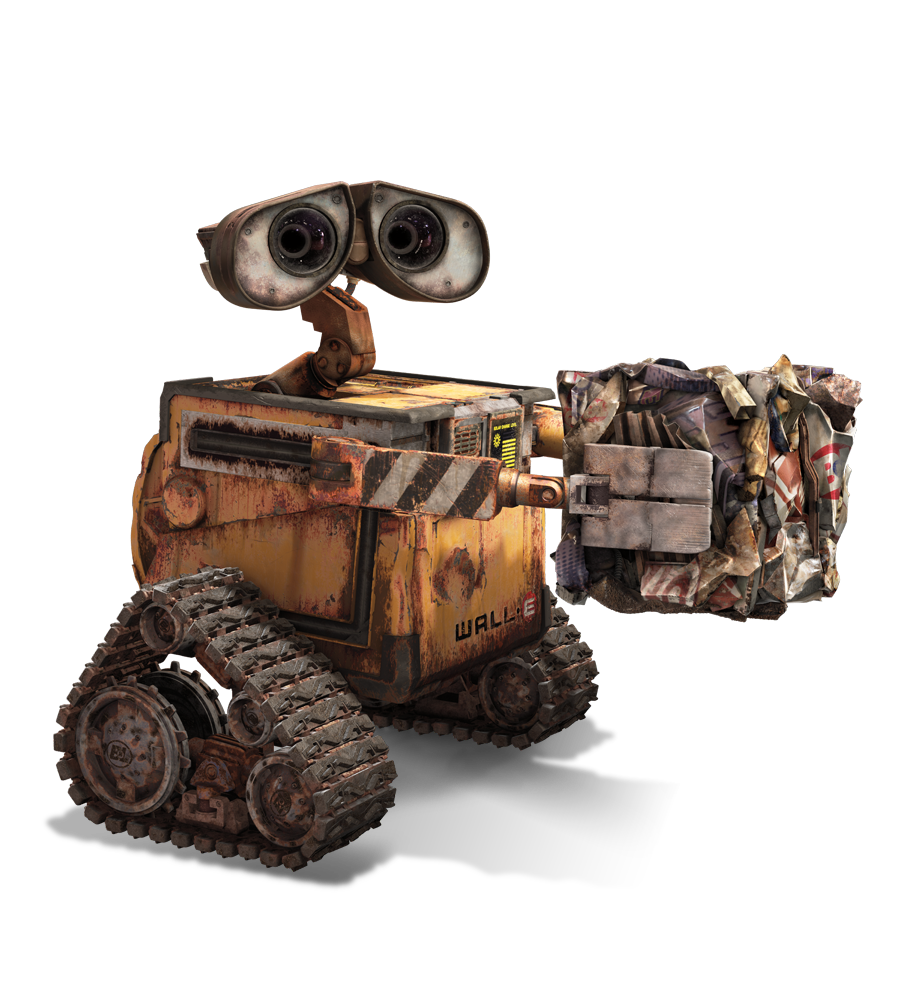
\includegraphics[height=3cm, keepaspectratio]{images/walle.png}
        \end{center}
        Il comando \texttt{\textbf{tar}} ci permette di aggregare file e/o cartelle in un archivio (con estensione .tar).
        
        \vspace{0.5cm}

        Opzionalmente, è possibile comprimere gli archivi facendoli
        passare per un filtro di compressione (\textbf{bzip, bzip2, xz}) in
        modo esplicito (usando una pipe) oppure in modo implicito (utilizzando le opzioni \textbf{-z},\textbf{-j} o \textbf{-J}).
    \end{frame}

    \begin{frame}{Tar: sintassi}
        \begin{block}{tar}
            \small
            Sintassi: \texttt{\textbf{tar [-c|-x|-t] [-z|-j|-J] [-v] [-f archive] [pathname]}}
            
            \begin{itemize}
                \item \texttt{\textbf{-c}}: crea un archivio
                \item \texttt{\textbf{-x}}: estrae un archivio
                \item \texttt{\textbf{-t}}: elenca il contenuto di un archivio
                \item \texttt{\textbf{-v}}: mostra il progresso (modalità \textbf{verbose})
                \item \texttt{\textbf{-z/-j/-J}}: comprime l'archivio con \textbf{gzip}/\textbf{bzip2}/\textbf{xz}
                \item \texttt{\textbf{-f archive}}: specifica l'archivio
                \item \texttt{\textbf{pathname}}: file e/o directory da comprimere
            \end{itemize}
        \end{block}
    \end{frame}

    \begin{frame}{Tar: esempi}
        \scriptsize
        \begin{exampleblock}{}
            \texttt{\$ tar -c -v -f prova.tar *.tex *.pdf images/} \\
            \texttt{
            slides.tex \\
                slides.pdf \\
                images/ \\
                images/penguin.pdf \\
                images/penguin2.pdf \\
                ...
            }

            \vspace{0.25cm}

            \texttt{\$ tar x -f prova.tar}

            \texttt{\$ tar cjf prova2.tar.bz2 images/ *.pdf}
            
            \vspace{0.25cm}

            \texttt{\$ bzcat prova2.tar.bz2 | tar tv}

            \texttt{drwxr-xr-x davide/davide     0 2023-06-04 10:07 images/ \\
            -rw-r-{}-r-{}- davide/davide  2336 2023-03-28 17:42 images/penguin.pdf \\
            -rw-r-{}-r-{}- davide/davide  1886 2023-03-28 17:44 images/penguin2.pdf
            }

            \vspace{0.25cm}

            \texttt{\$ tar c images/ *.pdf | gzip > prova3.tar.gz}
        \end{exampleblock}
    \end{frame}

    \begin{frame}{Alias}
        \begin{block}{alias}
            \small
            Sintassi: \texttt{\textbf{alias [name[=value]]}}

            Il comando \texttt{\textbf{alias}} permette di associare a nomi propri sequenze arbitrarie
            di comandi e opzioni. Inoltre,

            \begin{itemize}
                \item \texttt{\textbf{alias}} (senza parametri): restituisce la lista degli alias attualmente attivi
                \item \texttt{\textbf{alias name}}: restituisce l'associazione attuale per \texttt{\textbf{name}}
                \item \texttt{\textbf{unalias name}}: rimuove l'alias \texttt{\textbf{name}}
            \end{itemize}
        \end{block}

        \begin{exampleblock}{Esempio}
            \scriptsize

            \texttt{\$ alias ll=`ls -l'}
            
            \texttt{\$ ll /}

            \texttt{lrwxrwxrwx   1 root root    7 31 gen 21.51 bin -> usr/bin \\
            drwxr-xr-x   1 root root  180 31 mag 10.56 boot \\
            drwxr-xr-x  21 root root 4,1K  4 giu 08.04 dev \\
            ...
            }
        \end{exampleblock}
    \end{frame}

    \begin{frame}{Modalità di esecuzione}
        Esistono varie modalità di esecuzione dei comandi sulla shell.
        
        La più semplice consiste nell'invocazione di un singolo comando.

        Ogni comando restituisce un \textbf{exit status} che
        rappresenta l'esito dell'esecuzione del comando stesso.

        \vspace{0.5cm}

        L'\textbf{exit status} è un intero nel range $[0,255]$.
        
        Questo è posto a:
        
        \hspace{1cm} $\textbf{0}$: se l'esecuzione è riuscita con successivo

        \hspace{1cm} $\textbf{> 0}$: se l'esecuzione è fallita

        \vspace{0.5cm}

        I valori nel range $[1,255]$ sono utili per specificare all'utente il tipo di errore
        riportato durante l'esecuzione.
    \end{frame}

    \begin{frame}{\textit{Simple Command Execution}}
        \centering
        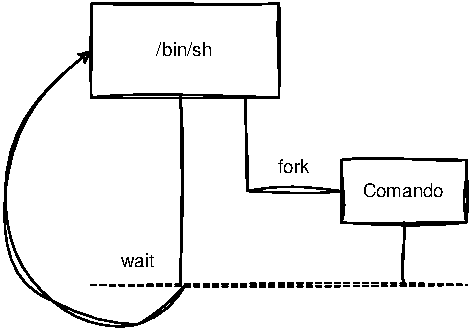
\includegraphics[height=7cm,keepaspectratio]{images/sce.pdf}
    \end{frame}

    \begin{frame}{\textit{Pipeline}}
        \centering
        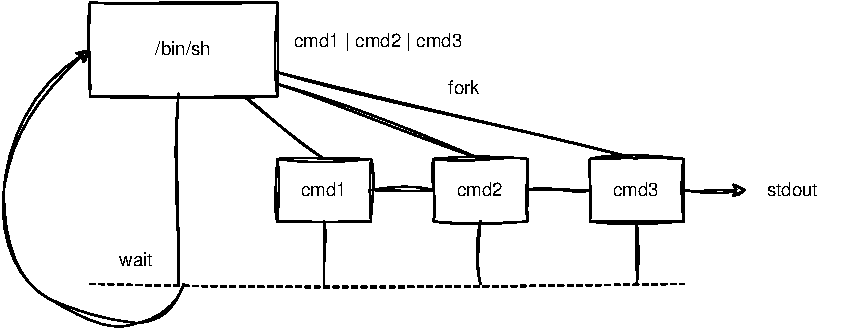
\includegraphics[height=4.4cm,keepaspectratio]{images/pipeline.pdf}
    \end{frame}

    \begin{frame}{\textit{List of command}}
        La lista di comandi permette di raggruppare una sequenza di comandi.
        La sintassi per l'invocazione è la seguente
        \begin{center}
            \texttt{\textbf{comando1 [; comando2...]}}
        \end{center}

        L'\textbf{exit status} della sequenza è uguale a quello dell'ultimo comando
        presente nella lista.

        \vspace{1cm}

        \begin{exampleblock}{Esempio}
            \footnotesize
            \texttt{\$ echo -n "Via "; echo -n "del "; echo "campo"}
            
            \texttt{Via del campo}
        \end{exampleblock}
    \end{frame}

    \begin{frame}{\textit{List of command}}
        \centering
        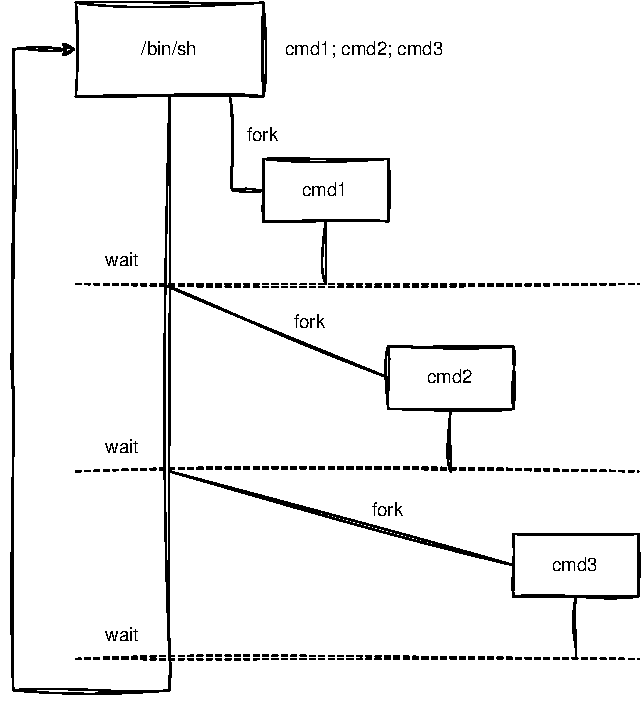
\includegraphics[height=7.5cm, keepaspectratio]{images/loc.pdf}
    \end{frame}

    \begin{frame}{\textit{List of command}}
        Nelle sequenze di comandi è possibile utilizzare gli operatori
        condizionali \textbf{\&\&} e \textbf{||}. La semantica è la seguente:
        \begin{itemize}
            \item \texttt{\textbf{c1 \&\& c2}}: \texttt{c2} viene eseguito se e solo se l'exit status di \texttt{c1} è 0.
            \item \texttt{\textbf{c1 || c2}}: \texttt{c2} viene eseguito se e solo se l'exit status di \texttt{c1} è diverso da 0.
        \end{itemize}

        L'exit status di una lista condizionata è uguale all'exit status dell'ultimo comando eseguito.

        \begin{exampleblock}{Esempio}
            \footnotesize

            \texttt{\$ cat fileinesistente \&\&  echo fatto}

            \texttt{cat: fileinesistente: File o directory non esistente}

            \vspace{0.5cm}
            
            \texttt{\$ cat fileinesistente || echo errore}

            \texttt{cat: fileinesistente: File o directory non esistente}

            \texttt{errore}
        \end{exampleblock}
    \end{frame}

    \begin{frame}{\textit{Asynchronous execution}}
        Un comando può essere eseguito in \textbf{background} usando la sintassi
        \begin{center}
            \texttt{\textbf{comando \&}}
        \end{center}

        \vspace{0.5cm}

        Inoltre, un processo in \textbf{foreground} può essere mandato
        in background interattivamente attraverso la combinazione di tasti
        \textbf{CTRL + Z}. In questo caso però il processo sospeso.

        \vspace{0.5cm}

        Questo può essere riportato in foreground utilizzando il comando \texttt{\textbf{fg}}.
    \end{frame}

    \begin{frame}{Controllo dei \textit{job}}
        La shell associa ad ogni comando un \textbf{job}. Ogni job
        viene identificato univocamente da un numero, detto \textbf{jobnumber}.

        Proprio per questo, quando un comando viene eseguito in modo asincrono, la shell restituisce il seguente output
        \begin{center}
            \texttt{[jobnumber] PID}
        \end{center}

        Per controllare i job è possibile utilizzare i seguenti comandi:

        \begin{itemize}
            \item \textbf{jobs}: visualizza i job attivi e il loro stato
            \item \textbf{bg}: manda in background un job
            \item \textbf{fg}: porta in foreground un job
            \item \textbf{kill}: invia un segnale ad un job
        \end{itemize}
    \end{frame}

    \section{BASH}

    % \begin{frame}{Quoting}
    %     Il meccanismo del \textbf{quoting} serve ad eliminare il metasignificato
    %     ad alcuni caratteri. Questo può essere di tre tipi:
    %     \begin{itemize}
    %         \item \textbf{\textbackslash} (\textit{backslash}): elimina il metasignificato del carattere seguente
    %         \item \textbf{` '} (\textit{single quote}): elimina il metasignificato da tutti i caratteri contenuti al suo interno
    %         \item \textbf{`` ''} (\textit{double quote}): elimina il metasignificato da tutti i caratteri contenuti al suo interno ad eccezione di \textbf{\$}, \textbf{`} e \textbf{\textbackslash}.
    %     \end{itemize}

    %     \begin{exampleblock}{Esempi}
    %         \scriptsize
    %         \texttt{\$ echo \$PATH}
            
    %         \texttt{/usr/local/bin:/usr/bin:/usr/local/sbin...}

    %         \texttt{\$ echo \textbackslash\$PATH}

    %         \texttt{\$PATH}

    %         \vspace{0.25cm}

    %         \texttt{\$ echo "Il mio nome è \$USER e ho 5\$.}

    %         \texttt{Il mio nome è davide e ho 5\$.}
    %     \end{exampleblock}
    % \end{frame}


    
\end{document}
